\documentclass[a4paper,12pt]{report}
\usepackage[spanish,mexico]{babel}
\usepackage[utf8]{inputenc}
\usepackage[T1]{fontenc}
\usepackage{amsmath}
\usepackage{amssymb}
\usepackage{wasysym}
\usepackage[dvipsnames,pdftex]{color}
\usepackage[colorinlistoftodos]{todonotes}
%\usepackage{helvet}
%\renewcommand{\familydefault}{\sfdefault}
\setlength{\oddsidemargin}{0in}
\usepackage{here}
\usepackage{geometry}
 \setlength{\textwidth}{6.4in}
 \setlength{\topmargin}{0in}
 \setlength{\voffset}{-0.6in}
 \setlength{\hoffset}{-0.2in}
 \setlength{\textheight}{9.7in}
 \setlength{\topskip}{0in}
 \setlength{\parskip}{2ex}
 \renewcommand{\baselinestretch}{1.5}
\usepackage{diagbox}
\usepackage{array}
\usepackage{listings}
\usepackage{caption}
%%% comandos definidos por el usuario
\begin{document}
\setcounter{page}{1}
\pagenumbering{roman}
\thispagestyle{empty}
\begin{center}
{\huge UNIVERSIDAD NACIONAL DE INGENIERÍA}\\[0.9cm]
{\Large FACULTAD DE INGENIERÍA MECÁNICA}\\[0.6in]
\end{center}
\begin{figure}[h]
\begin{center}

\includegraphics[scale=0.33]{logoUNI.png}
\vspace{0cm}
\end{center}
\end{figure}
\vspace{0.5cm}
\begin{center}
INFORME DE LABORATORIO\\
LABORATORIO DE INGENIERÍA MECÁNICA\\[14mm]
{\large MEDICIÓN DE FLUJO}\\[10mm]
\vfill
LIMA - PERÚ \hfill OCTUBRE 2019
\end{center}
\newpage
\thispagestyle{empty}
\begin{center}
{\Huge MEDICIÓN DE FLUJO}\\[0.7cm]
\small ENTREGADO:\\[0.3cm]
\small 06 OCTUBRE 2019\\[2.9cm]
\end{center}
\begin{flushleft}
{\large ALUMNOS:}\\[2cm]
\end{flushleft}
\begin{tabular}{c@{\hspace{0.5in}}c}
\rule[1pt]{2.6in}{1pt}&\rule[1pt]{2.6in}{1pt}\\
Carranza Zavala David, 20174065E & Huaroto Villavicencio Josue, 20174070I\\[2.5cm]
\rule[1pt]{2.6in}{1pt}&\rule[1pt]{2.6in}{1pt}\\
Landeo Sosa Bruno, 20172024J & Lino Carbajal Franklin, 20110146D\\[2.5cm]
\rule[1pt]{2.6in}{1pt}&\rule[1pt]{2.6in}{1pt}\\
Quesquen Vitor Angel, 20170270C & Sotelo Cavero Sergio, 20172125K\\[2.5cm]
\end{tabular}
%\begin{center}
%\begin{tabular}{c@{\hspace{0.5in}}c}
%\rule[1pt]{3.14in}{1pt}\\
%Sotelo Cavero Sergio, 20172125K% & Nombre 5, 2017 \\[1.5cm]
%\end{tabular}
%\end{center}
%\begin{center}
%\begin{tabular}{c@{\hspace{0.6in}}c}
%\rule[1pt]{3.14in}{1pt}\\
%Huaroto Villavicencio Josué, 20174070I \\[2.5cm]
%\rule[1pt]{3.14in}{1pt}\\
%Landeo Sosa Bruno, 20172024J \\[2.5cm]
%\rule[1pt]{3.14in}{1pt}\\
%Quesquen Vitor Angel, 2017 \\[2.5cm]
%\rule[1pt]{3.14in}{1pt}\\
%Sotelo Cavero Sergio, 20172125K
%\end{tabular}
%\end{center}
%\begin{center}
%\begin{tabular}{c}
%\rule[1pt]{3.14in}{1pt}\\
%Huaroto Villavicencio Josué, 20174070I \\[2.5cm]
%\end{tabular}
%\end{center}

%\rule[1pt]{3.14in}{1pt}\\
%Maguiña Amaya Wladimir, 20172019F \\[3cm]
%\rule[1pt]{3.14in}{1pt}\\
%Luis Sosa Jose, 19774147I \\[3cm]
%\rule[1pt]{3.14in}{1pt}\\
%Sotelo Cavero Sergio, 20172125K
%\end{tabular}
%\end{center}
%\\[0.7cm]
{\large PROFESOR:} \\[0.6cm]
\begin{center}
\begin{tabular}{c}
\rule[3pt]{4.8in}{1pt}\\[1pt]
ING. MORALES TAQUIRI OSWALDO
\end{tabular}
\end{center}
\vfill
%\newpage
%\begin{center}
%{\Large \bf{RESUMEN}}
%\end{center}
\newpage
\tableofcontents
%\listoffigures
%\addcontentsline{toc}{chapter}{Índice de figuras}
\newpage
\pagenumbering{arabic} %%% esto es para regresar el modo de numeración a numeración arábiga
\setcounter{page}{1}  %%% empezamos en página 1
%\part{Introducción}
\chapter{Objetivos}
\begin{enumerate}
\item El objetivo de la medición con Venturi es determinar un factor que nos permita comparar resultados teóricos con los reales, recordemos que hay pérdidas en las tuberías y pues, este factor lo considerará.
\item Comparar la exactitud de este tubo, cuya instalación es cara, vs otro instrumento que tiene una instalación barata. 
\item Calcular los coeficientes de descargas para la placa y el venturímetro.
\end{enumerate}
\chapter{Cálculos y resultados}
\section{Estudio del flujo en vertedero triangular}
Cuadro con los datos obtenidos en esta parte experimental:
\begin{center}
\begin{tabular}{|c|c|c|c|c|c|}
\hline 
Medición & Altura Tanque & Altura Flotador & Tiempo (seg) & Volumen (ml) & Caudal (ml/s) \\ 
\hline 
1 & 20.5 cm & 0.4 in & 15 & 670 & 44.6667 \\ 
\hline 
2 & 45 cm & 0.49 in & 30.5 & 1954 & 64.0656 \\ 
\hline 
3 & 57.5 cm & 0.5 in & 15.33 & 1090 & 71.1024 \\ 
\hline 
4 & 64 cm & 0.75 in & 15.18 & 1160 & 76.4163 \\ 
\hline 
\end{tabular} 
\end{center}
\subsection{Relación entre el tanque y el caudal en la salida}
Conocemos la relación teorica existente entre la altura $(h)$ de agua presente en el tanque y la velocidad de salida por un orificio en la parte inferior del tanque. Esta relación se representa mediante la formula:
$$
V_{\mathrm{salida}} = \sqrt{2gh}
$$
Entonces para un área de salida constante que desconocemos debería cumplirse que la relación caudal/velocidad debe ser lineal:
\begin{figure}[H]
\centering
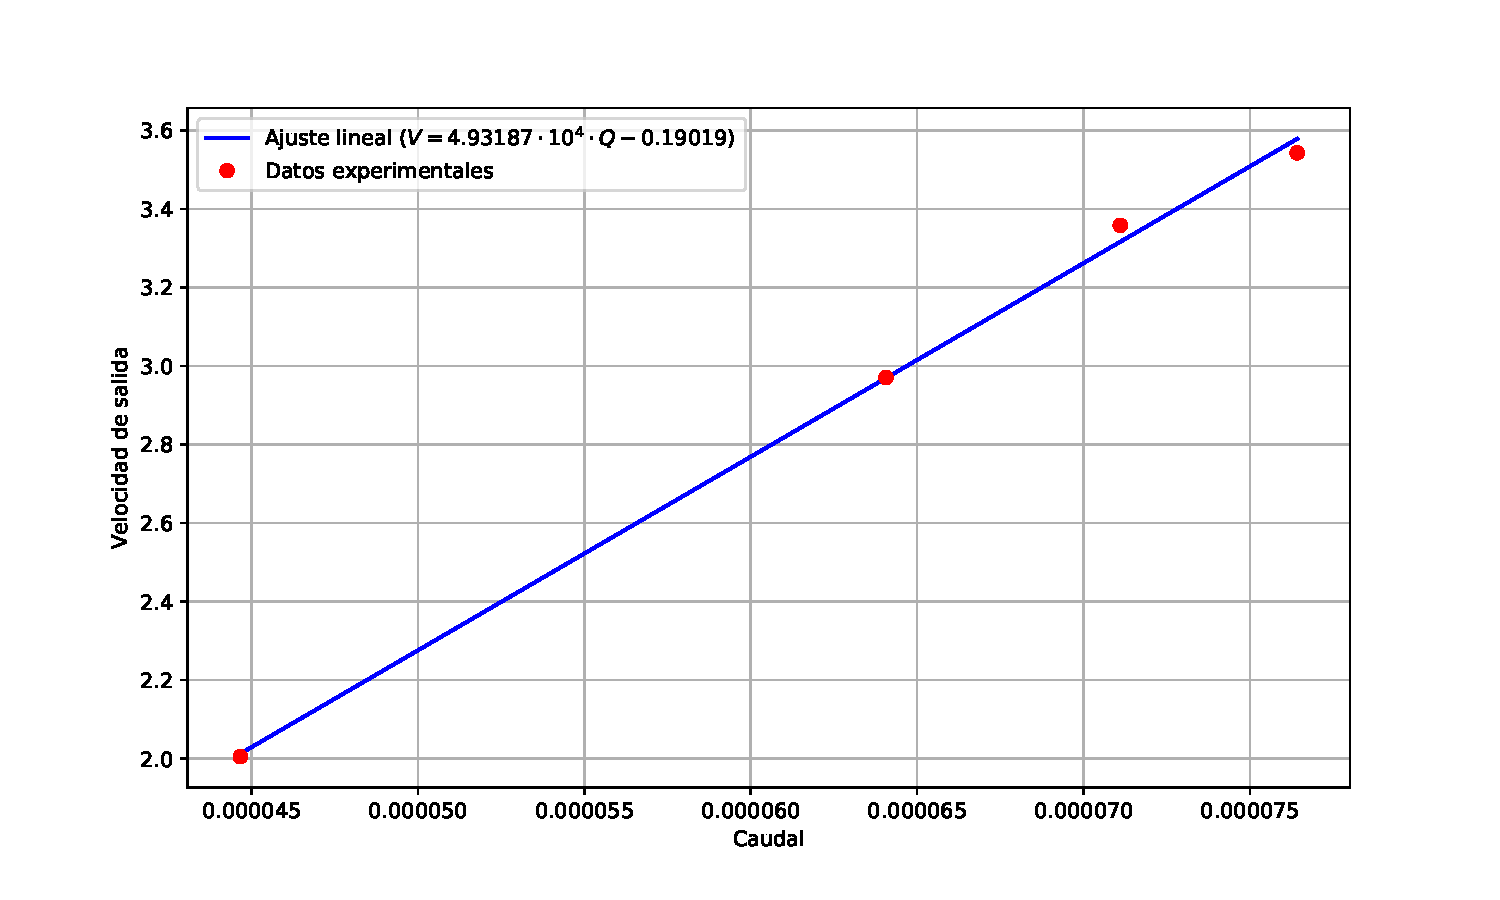
\includegraphics[scale=0.7]{velocidadcaudal.pdf}
\end{figure}
De esta grafica podemos deducir que el área de salida del orificio es de $2.02763\cdot 10^{-5} \mathrm{m^{2}}$ aproximadamente.
\subsection{Relación entre el caudal y la altura del medidor flotante para el perfil triangular}
De los libros y manuales de hidráulica se puede obtener la siguiente formula para un vertedero triangular con ángulo de $90^{\circ}$:
$$
Q_{teorico} = \frac{8}{15} \sqrt{2g} h^{5/2}
$$
Esta expresión fue estudiada con mayor profundidad y James Thompson la replanteo considerando un coeficiente de descarga, lo que resulta en:
$$
Q_{real} = 0.593\,Q_{teorico} = 1.4\,h^{5/2}
$$
Con $Q$ en m$^{3}$/s y $h$ en metros. Además, esta formula sirve para valores de $h$ entre 5 y 18\,cm. Puesto que el coeficiente de descarga depende de las condiciones de ensayo y de los materiales; varios autores realizaron sus propios ensayos y obtuvieron distintas constantes cercanas al valor de Thompson (1.4$\pm$0.15 y 2.5$\pm$0.2 aproximadamente). En general se puede deducir que el caudal depende únicamente de la altura por encima del vértice del triángulo o también llamado carga de agua.
$$
Q_{h} = K\cdot h^{n}
$$
Para nuestro ensayo obtuvimos los siguientes datos de caudal y carga de agua (Altura del flotador):
\begin{center}
\begin{tabular}{|c|c|}
\hline 
Carga de agua (m)
 & Caudal (m$^{3}$/s) \\ 
\hline 
0.01016 & 4.4667e-05 \\ 
\hline 
0.012446 & 6.406557e-05 \\ 
\hline 
0.0127 &  7.110241e-05 \\ 
\hline 
0.01905 &  7.64163e-05 \\ 
\hline 
\end{tabular} 
\end{center}
\begin{figure}[H]
\centering
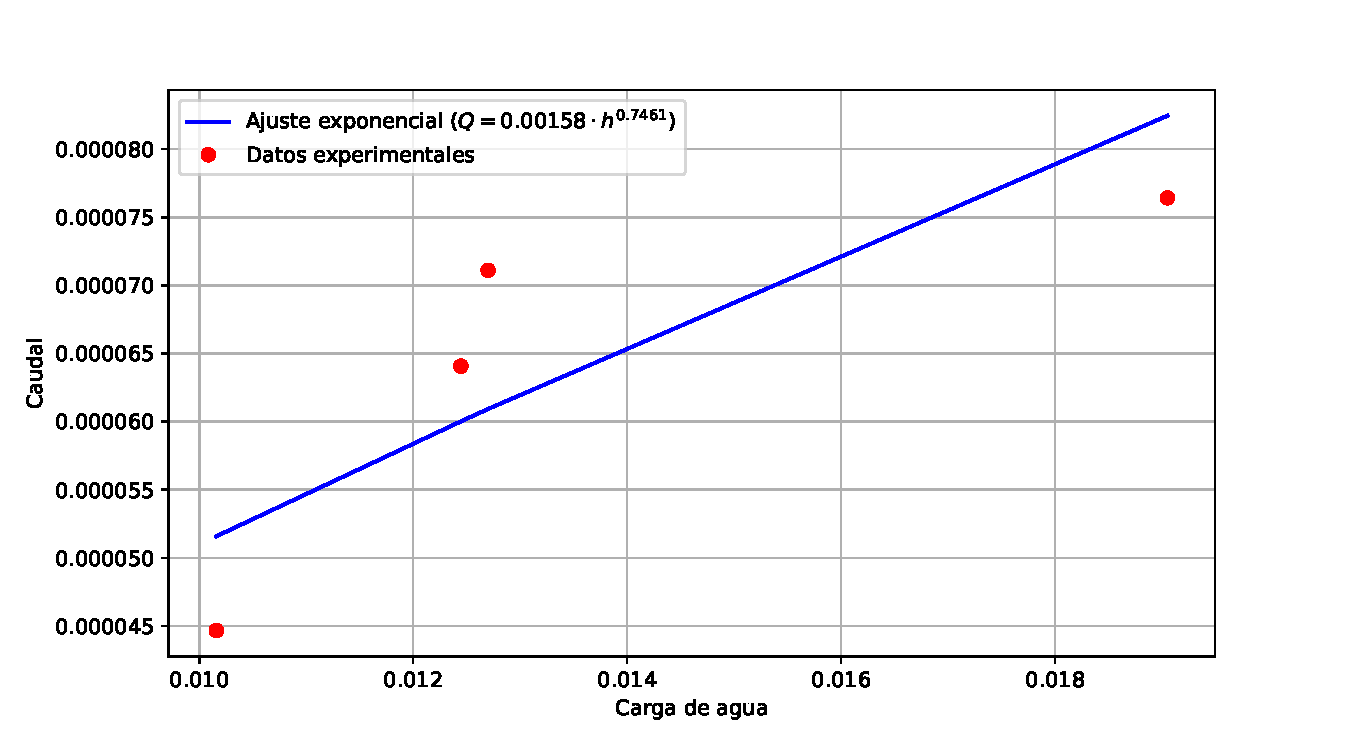
\includegraphics[scale=0.75]{caudalaltura.pdf}
\end{figure}
\section{Tubo de Venturi}
\begin{figure}[H]
\centering
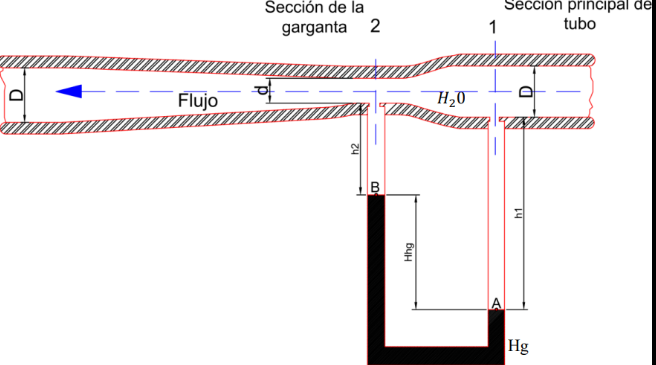
\includegraphics[scale=0.5]{ser1.png}
\end{figure}
Primera toma:
$$
Q_{1} = \frac{10\,\mathrm{L}}{9.7\,\mathrm{s}} = 0.0010309 \, \mathrm{m^{3}/s} \mathrm{real} \hspace{40pt} \Delta H = 0.101\,\mathrm{m}
$$
$$
v_{2} = 5.3559439\,\mathrm{m/s} \longrightarrow Q_{2} = 0.001526\,\mathrm{m^{3}/s}
$$
Segunda toma
$$
Q_{2} = \frac{10\,\mathrm{L}}{24.215\,\mathrm{s}} = 0.000412967 \, \mathrm{m^{3}/s} \mathrm{real} \hspace{40pt} \Delta H = 0.022\,\mathrm{m}
$$
$$
v_{2} = 2.49969\,\mathrm{m/s} \longrightarrow Q_{2} = 0.00071247\,\mathbb{m^{3}/s}
$$
Ahora procederemos a calcular los coeficientes de descarga que tiene cada muestra la cual se calculará bajo esta expresión:
$$
Cd_{1} = \frac{Q_{\mathrm{real}}}{Q_{\text{teórico}}} = 0.6753 \hspace{40pt} Cd_{2} = 0.5796
$$
Entonces el $Cd_{\mathrm{prom}} = 0.6274$.
\section{Placa orificio}
\subsection{Procedimiento}
\begin{enumerate}
\item Activar las bombas
\item De la misma manera que el ensayo de Venturi, se verifican que existan cantidades de agua en el tubo, si existiera, se cuantifican para corregir posibles errores.
\item Se are la llave de agua y se anotan las diferentes alturas en los niveles de mercurio
\item La medición del caudal se hace de la misma manera que con la experiencia de Venturi.
\item Cuando se inicie la medición del caudal, se cierra la llave del tanque, luego se abre la llave de descarga para proseguir con las mediciones.
\end{enumerate}
\subsection{Cálculos y resultados}
Se mostrará en detalle los cálculos y resultados del coeficiente de descarga ($Cd$) de la tubería placa orificio concéntrica interna al tubo.
\begin{figure}[H]
\centering
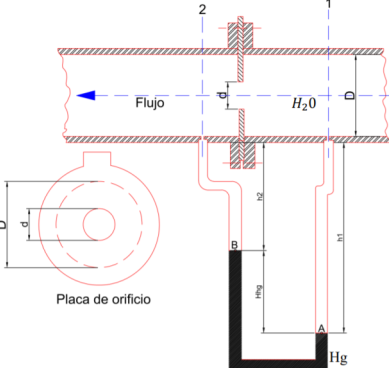
\includegraphics[scale=0.6]{fr1.png}
\end{figure}
\begin{center}
\begin{tabular}{|c|c|c|c|}
\hline 
$D$ (Diámetro mayor) & $d$ (Diámetro menor) & $A_{D}$ & $A_{d}$ \\ 
\hline 
5/4 in & 3/4 in & $7.917\cdot 10^{-4} \mathrm{m^{2}} $ & $2.85\cdot 10^{-4} \mathrm{m^{2}} $ \\ 
\hline 
\end{tabular} 
\end{center}
Datos obtenidos en el laboratorio:
$$
T_{amb} = 20^{\circ}\mathrm{C} \hspace{20pt} \rho_{\mathrm{agua}} = 998 \mathrm{kg/m^{3}} \hspace{20pt} \gamma_{\mathrm{agua}} = 9790\,\mathrm{N/m^{3}} \hspace{20pt} \mu_{\mathrm{agua}} = 1.02\cdot 10^{3}\;\mathrm{Pa \cdot s}
$$
\begin{center}
\begin{tabular}{|c|c|c|c|c|c|c|}
\hline 
Medición & $\Delta\,h$ (cm\,Hg) & Volumen (L) & $t_{1}$ & $t_{2}$ & $Q_{real}$ (m$^{3}$/s) \\ 
\hline 
1 & 3 & 10 & 17.5 s & 17.85 s & 0.0005657 \\ 
\hline 
2 & 7.5 & 10 & 10.14 s & 9.54 s & 0.00102 \\ 
\hline 
\end{tabular} 
\end{center}
\subsubsection{Medición de la velocidad del fluido}
Para ello se aplicará tres restricciones:
\begin{itemize}
\item Aplicar la ecuación de Bernoulli entre los puntos (1) y (2).
\item Usar la ecuación de continuidad, por ser fluido incompresible entre los puntos (1) y (2). 
\item Análisis en el manómetro de mercurio entre los puntos (1) y (2).
\item Se obtendrá la siguiente expresión matemática:
\end{itemize}
$$
v_{2} = \sqrt{\frac{2gh_{Hg}\left(\frac{\rho_{Hg}}{\rho_{\mathrm{agua}}}-1\right)}{1-\left(\frac{d}{D}\right)^{4}}} \hspace{80pt} Q_{\mathrm{teorico}} = \frac{v_{2}\,\pi\,d^{2}}{4}
$$
Para la medición 1:
$$
v_{2} = 2.9152\,\mathrm{m/s} \hspace{60pt} Q_{\mathrm{teorico}} = 8.3\cdot 10^{-4}\,\mathrm{m^{3}/s}
$$
Para la medición 2:
$$
v_{2} = 4.609\,\mathrm{m/s} \hspace{60pt} Q_{\mathrm{teorico}} = 1.3137\cdot 10^{-3}\,\mathrm{m^{3}/s}
$$
Al obtener los dos caudales para ambas mediciones ($Q_{t}$,$Q_{r}$) se procede a calcular el coeficiente de descarga ($Cd$):
$$
Cd_{1} = \frac{Q_{\mathrm{real}}}{Q_{\mathrm{teorico}}} = 0.6867 \hspace{60pt} Cd_{2} = 0.7765
$$
De una T = 20$^{\circ}$C según indica las propiedades del agua y los datos obtenido en cálculos anteriores podemos calcular el  número de Reynold (Re):
$$
\mathrm{Re}_{1} = 54336.755 \hspace{40pt} \mathrm{Re}_{2} = 85907.69320
$$
Se procederá a obtener los promedios del $Cd$ y Re:
$$
Cd_{\mathrm{prom}} = 0.7316 \hspace{40pt} \mathrm{Re} = 70122.22
$$
Según tablas, $Cd = 0.65$:
$$
\%\mathrm{error} = \frac{0.7316-0.65}{0.7316} = 11.1535\%
$$
Al tener un \% error apreciable indica que para un Re > 4000 el flujo es turbulento, pero solo en la parte cercana al orificio, ya que después ello regresara a su estado laminar a medida que disminuye la velocidad y se tome constante.
\chapter{Conclusiones}
\begin{enumerate}
\item Se concluye que definitivamente hay pérdidas, pues los caudales son mayores teóricamente.
\item Es de utilidad tener el valor del coeficiente de descarga para estimar el caudal que se obtendrá al usar cualquier dispositivo que pueda afectar el caudal.
\end{enumerate}
\chapter*{Anexos}
\begin{figure}[H]
\centering
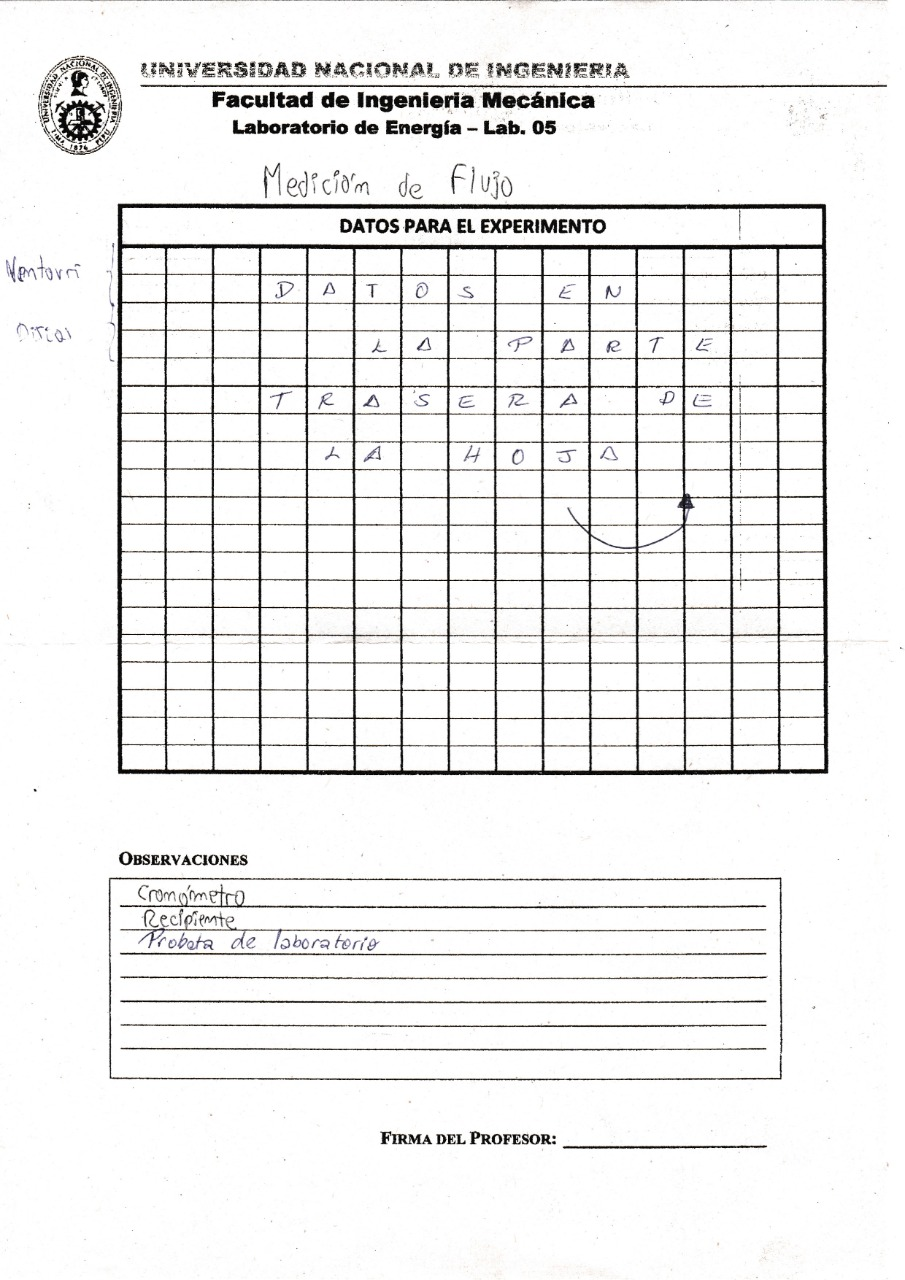
\includegraphics[scale=0.45]{datos1.jpeg}
\end{figure}
\begin{figure}[H]
\centering
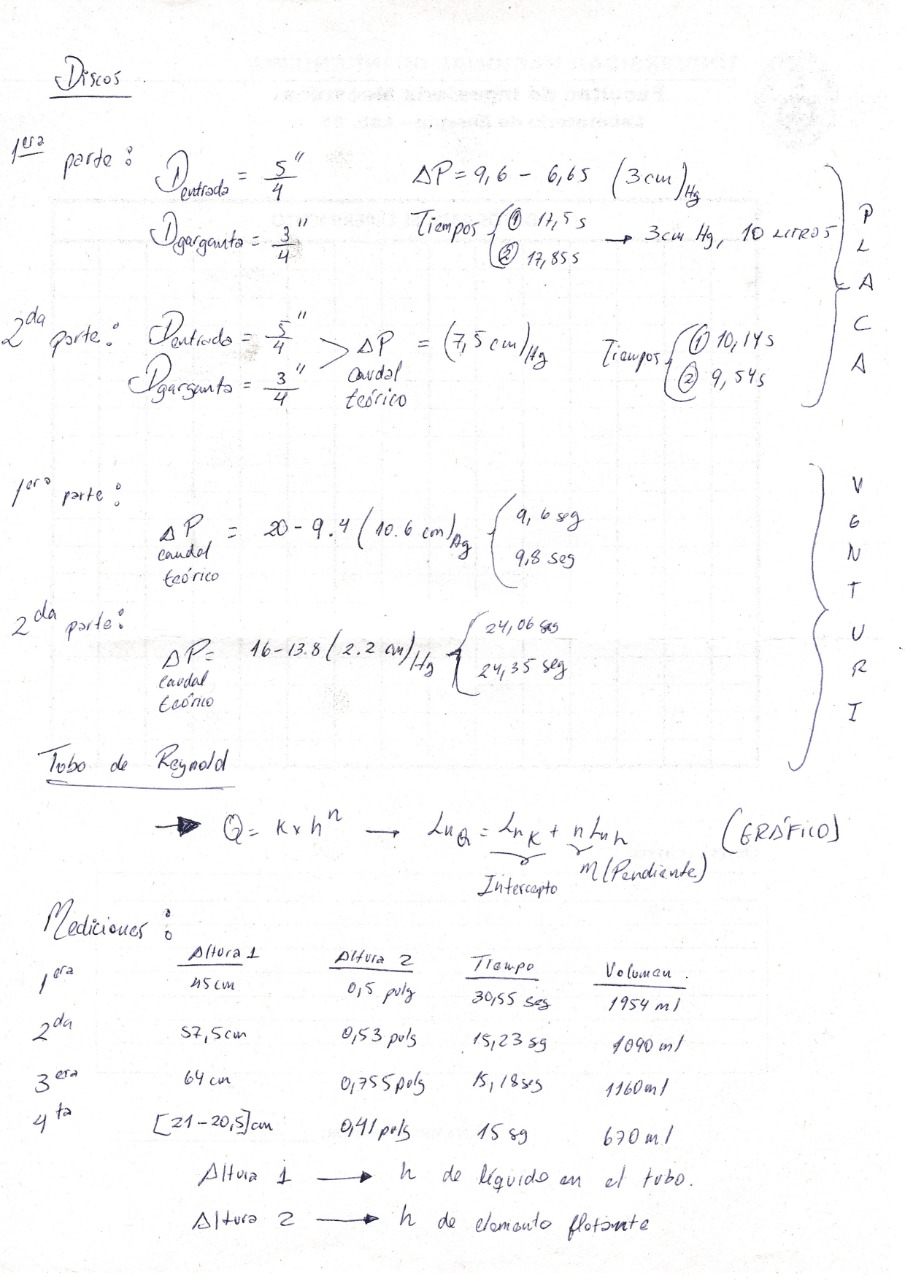
\includegraphics[scale=0.5]{datos2.jpeg}
\end{figure}
\begin{figure}[H]
\centering
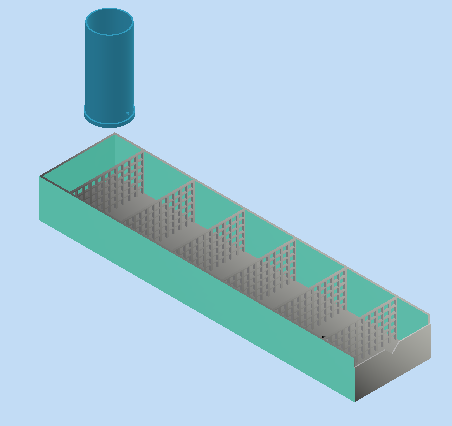
\includegraphics[scale=0.9]{anexo1.png}
\end{figure}
\begin{figure}[H]
\centering
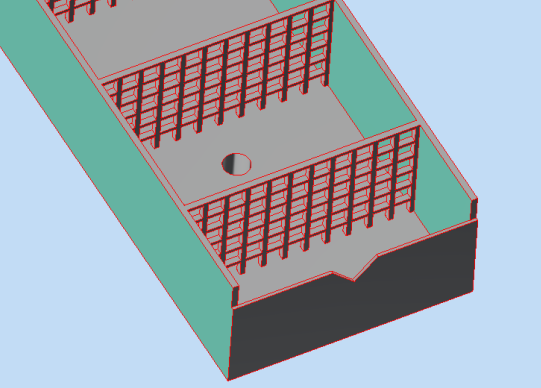
\includegraphics[scale=0.75]{anexo2.png}
\end{figure}
\begin{figure}[H]
\centering
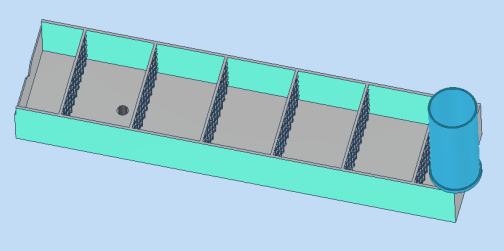
\includegraphics[scale=0.9]{anexo3.png}
\end{figure}
\begin{thebibliography}{99}  %%%este es un contador para el número de bibliografías utilizados.
\addcontentsline{toc}{chapter}{Bibliograf\'{\i}a} %%% Para introducir la bibliografía en el índice.
%\bibitem{Rahman}{Rahman,Aminur y Doe, Hidekazu; ``Ion transfer of tetraalkylammonium cations at an interface between 
%frozen aqueous solution and 1,2-dichloroethane".{\em{Journal of Electroanalytical Chemistry}} {\bfseries 424},159,(1997).}
\bibitem{Gro}{Chow, V.``Open Channel Hydraulics''.{\em{McGraw-Hill}}}
\bibitem{Gro}{Domínguez, F.``Hidráulica''.}
\bibitem{Ding}{Guevara, Robert (2009).``Manual de prácticas de laboratorio de energía II''.}
\bibitem{AL}{Mott, R. ``Mecánica de fluidos''.\em{Prentice-Hall}}
%\bibitem{AL}{Alonso, Jose M. ``Técnicas de mecanizado 1". {\em{Paraninfo}} {\bfseries España-Madrid}, 6-20, (2001).}
%\bibitem{Samec2}{Samec Z., Lhotsky A., Jänchenová H., y Marecek, V. ``Interfacial tension and impedance measurements
%of interfaces between two inmiscible electrolyte solutions". {\em{Journal of Electroanalytical Chemistry}} {\bfseries
%43}, 47, (2000).}
%\bibitem{Day}{Day R.A. y Underwood A.L. {\textit{Química Analítica Cuantitativa}},5ºed. Prentice-Hall, México, 1998. 45-48.}
%\bibitem{Keyser}{Farah Abud, Michel. ``Determinación de la vida útil en herramientales de corte endurecido por el proceso de borurización en pasta''. {\em{Instituto tecnológico y de estudios superiores de Monterrey}}}
%\bibitem{Zolotorevski}{Escalona, I. ``Máquinas: herramientas por arranque de viruta.''.{\em{El Cid Editor.}}}
%\bibitem{Lasheras}{Lasheras. ``Tecnología de los Materiales Industriales''.} 
%\bibitem{Dieter}{Dieter. ``Metalurgia mecánica''.}
%\bibitem{Apraiz}{Apraiz, J. ``Tratamiento Térmico de los Aceros''.}
%\bibitem{Smith}{Smith, William F. y Ph.D. Hashemi, Javad ``Ciencia e ingeniería de materiales". {\em{
%Madrid: McGraw-Hill, Interamericana de España.}} 570, (2004).} 
%\bibitem{Callister}{Callister, William D. y Rethwisch, David G. ``Introducción a la ingeniería de los materiales''. %{\em{Barcelona Reverté.}}, 960, (2007).} 
%\bibitem{Askeland}{Askeland, Donald R., Pradeep P. Phulé y Wright, Wendelin J. ``Ciencia e ingeniería de los materiales''.{\em{México, D.F. Internacional Thomson Editores.}} {\textit{$6^{ta}$ edición}}, 1004, (2012).}
%\bibitem{HARDBANDING}{Tabla de conversión de escala de durezas. \begin{verbatim}http://%hardbandingsolutions.com/postle_sp/hardness.php
%\end{verbatim}}
%\bibitem{PR}{Termómetro bimetálico. \begin{verbatim}
%https://www.electrabel.es/el-funcionamiento-de-un-termometro-bimetalico/\end{verbatim}}
%\bibitem{PR}{Termómetro de inmersión total. \begin{verbatim}
%http://www.dilabsa.com/es/cual-es-la-diferencia-entre-los-termometros-
%de-inmersion-total-y-parcial/
%\end{verbatim}}
%\bibitem{PR}{Termómetro de inmersión parcial. \begin{verbatim}
%http://www.metas.com.mx/guiametas/La-Guia-MetAs-08-09-termometros-liquido-
%en-vidrio.pdf
%\end{verbatim}}
%\bibitem{HE}{Fresadora. \begin{verbatim} http://lizdenbow.blogspot.com/
%\end{verbatim}}
%\bibitem{ASTM}{Normas ASTM.}
%\bibitem{NTP}{Normas NTP.}
\end{thebibliography}
\end{document}